
\section{DDoS Attacks and BRO}\label{subsec:ddos-and-bro}
In this section, we will first define the notion of a DDoS attack by explaining the infrastructure. Then we elaborate on the most common DDoS attacks used according to Akamai's Q4 2017 report \cite{Akamai2017-4} and discuss their main characteristics. After this, we will discuss the syntax of the signature rules of the BRO SIDS.

\subsection{The DDoS Attack}
Figure \ref{fig:ddos-overview} shows the infrastructure of a DDoS attack. Actors involved in an attack are denoted by a letter (A-E) whereas data streams are denoted by numbers (1-5). 

A DDoS attack starts with an attacker (A). The attacker sends data needed to start the attack (1) to the Command and Control (C\&C) servers (B). The C\&C servers control the infected machines (C). The infected machines are also known under the name of bots. The C\&C servers plus the infected machines are more commonly known as a botnet. In case of the Ramnit botnet \cite{europol2015}, only the infected machines counted 3.2 million machines. When the C\&C servers receive a message from the attacker, they at their turn send a message (2) to the infected machines. At this point, two paths are used to get to the target machine (E). The first path possible is aiming the infected machines directly to the target (4). This means that traffic from the infected machines will go directly towards the target. The second path possible is using public services (D). This means that traffic from the infected machines will first go through a public service, like a DNS, to reach the target (5). 

A technique for an attacker to use the public services is by spoofing its IP. In this process, the attacker sends a request towards a public service where the packet's source IP is replaced by the one of the target.  This way the response of the service is reflected towards the target. A benefit for an attacker to use this path is that it is possible, due to the asymmetry between request and response sizes, to amplify once initial request.  In the next subsection, we describe various types of DDoS attacks and relate them to the architecture described above. 

\begin{figure}[H]
\centering
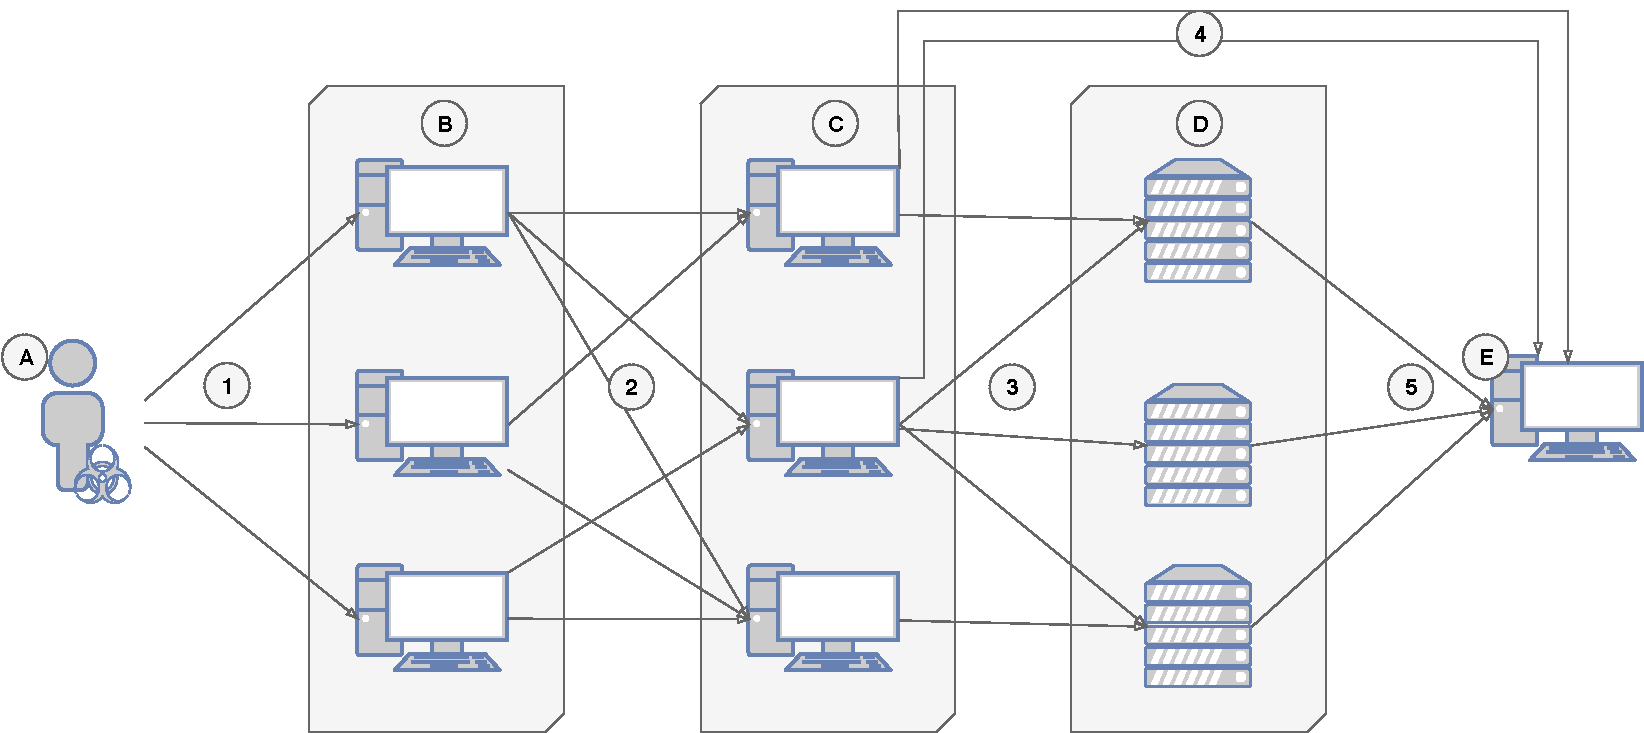
\includegraphics[width=\textwidth]{./images/ddos-overview.pdf}
\caption{Overview of DDoS attack infrastructure}
\end{figure}\label{fig:ddos-overview}

\subsection{Types of Attacks}\label{subsubsec:types-of-attacks}
In this subsection, we briefly elaborate on the top 10 most common types of DDoS attacks. This top 10 is retrieved from, at the time of writing, the latest report that gives an overview of the types of the most used DDoS attacks of Akamai \cite{Akamai2017-4}. Of each attack, we discuss which protocol is used and which mechanism is exploited. An overview of the main characteristics per attack type can be found in Table \ref{tab:attack-overview}.


\paragraph{UDP:}
The UDP attack exploits UDP protocol. The attack consists of sending a large number of packets to random ports of the target. Hereby the target machine will check if an application listens to this port and if not will reply with an ICMP Destination Unreachable (ICMP type 3) packet. At Figure \ref{fig:ddos-overview}, for this type of attack, path 4 is used.

\paragraph{UDP Fragment:}
The UDP Fragmentation attack exploits the fragmentation used in the IP protocol \cite{imperva}. When a packet is too big to be sent across a network link, it will be broken down into smaller packets and later on resembled again. In a UDP Fragmentation attack, UDP packets are sent which are larger than the maximum transmission unit (MTU), usually 1500 bytes, of the network thereby forcing fragmentation. This results in a higher number of packets than a normal UDP attack. At Figure \ref{fig:ddos-overview}, for this type of attack, path 4 is used.

\paragraph{DNS:}
The DNS attack exploits the public Domain Name System (DNS) services on the internet. DNS runs over UDP and is used to resolve IP addresses from website names. In a DNS attack, the attacker spoofs its IP replacing it by the one of the target. The DNS server sees the request as it came from the target and replies as if it were a normal request. This way of attacking allows an attacker to amplify its own bandwidth by using the asymmetry between request and response size. At Figure \ref{fig:ddos-overview}, for this type of attack, path 5 is used.

\paragraph{NTP:}
The NTP attack exploits the public Network Time Protocol (NTP) services on the internet. NTP uses the UDP protocol and allows for time synchronization between machines. This attack is similar to the DNS attack, but this time the NTP services are used instead of the DNS services. At Figure \ref{fig:ddos-overview}, for this type of attack, path 5 is used.

\paragraph{Chargen:}
The Chargen attack exploits the public Character Generator Protocol (Chargen) services. Once a Chargen service receives a packet via the UDP protocol, it responds by sending a datagram containing a random number between 0 and 512 characters long \cite{ietf1983}. The attack approach works the same as the NTP and DNS. At Figure \ref{fig:ddos-overview}, for this type of attack, path 5 is used.   

\paragraph{CLDAP:}
The CLDAP attack exploits the Connection-less Lightweight Directory Access Protocol (CLDAP). CLDAP runs over UDP and is designed to provide access to directories while not needing the resource requirements of the Directory Access Protocol (DAP) \cite{ietf1995}. The attack is similar to the DNS, NTP and Chargen attack. At Figure \ref{fig:ddos-overview}, for this type of attack, path 5 is used.

\paragraph{SYN:}
The SYN attack exploits the three-way handshake of TCP. During this attack, a large number of SYN packets are sent to the target machine. The target machine will respond by sending a SYN-ACK packet. The attacker at this point does not respond by sending an ACK packet, leaving the connection half initialized. This way the attacker keeps connections from being used by legitimate users. Compared to the attacks mentioned above, this one runs over TCP rather than UDP. At Figure \ref{fig:ddos-overview}, for this type of attack, path 4 is used.

\paragraph{SSDP:}
The SSDP attack exploits the Simple Service Discovery Protocol (SSDP). SSDP runs over UDP and is used to discover network services. The attack is similar to DNS, NTP and Chargen but at Figure \ref{fig:ddos-overview} the machines in D are for instance home routers, printers or other IOT devices rather than a dedicated server. 


\paragraph{ACK:}
The ACK attack exploits the TCP protocol. During this attack, a large number of ACK packets are sent towards the target. These ACKs do not belong to any connection and are therefore dropped at the target machine. This, however, does deplete resources of the target. At Figure \ref{fig:ddos-overview}, for this type of attack, path 4 is used.


\paragraph{HTTP:}
Rather than the attacks mentions above, the HTTP attack targets the application layer. The attack consists of sending a large number of HTTP requests (like GET, PUSH and POST) to the target, hereby depleting its resources. At Figure \ref{fig:ddos-overview}, for this type of attack, path 4 is used.



\begin{table}
\centering
\begin{tabular}{l | l}
Attack Type & Main Characteristics \\ \hline \hline
UDP Frag & IPv4 \&\& fragments \\ \hline
DNS & UDP \&\& src\_port==53 \&\& DNS\_query \&\& DNS\_type \\ \hline
CLDAP & UDP \&\& src\_port==389 \\ \hline
NTP & UDP \&\& src\_port==123 \\ \hline
UDP & UDP \\ \hline
Chargen & UDP \&\& src\_port==19 \\ \hline
SYN & TCP \&\& flag==SYN \\ \hline
SSDP & UDP \&\& src\_port==1900 \\ \hline
ACK & TCP \&\& flag==ACK \\ \hline
HTTP & HTTP \&\& HTTP\_request \&\& src\_port==80
\end{tabular}
\caption{\label{tab:attack-overview}Attack types main characteristic overview.}
\end{table}


\subsection{Bro Rule Syntax}\label{subsec:bro-rule-syntax} 
This section discusses the various parts used of Bro to implement the rule generation for the types of attacks discussed in Section \ref{subsubsec:types-of-attacks}. Bro's primary focus is on its scripting language.  With this language, one can define various analyzing scripts and detection policies. Besides the scripting language, Bro also offers also a signature language\footnote{\url{https://www.bro.org/sphinx/frameworks/signatures.html}}. This language is similar to Snort rules and relies on low-level pattern matching. In this section, first, an introduction to the signature language is given. Second, the signature language is applied to some of the attack types described in Section \ref{subsubsec:types-of-attacks}. Third and lastly, a brief explanation of the Bro scripting language is given.


The format of a signature is shown in Listing \ref{lst:signature-format}. As can be observed, each signature starts with the \emph{signature} keyword followed by a signature identifier. The body contains attributes. These attributes can be rules to match on. Besides rules, it is also possible to specify in the attributes whether an event must be raised when all attribute rules within a signature are matched for a specific package. Both possibilities will be explained further. 

\begin{lstlisting}[caption={Bro Signature Format}, label={lst:signature-format}]
signature [SIGNATURE-ID] {
  ATTRIBUTES 
}
\end{lstlisting}

An attribute rule follows the format \emph{KEYWORD CMP VALUE}. Here the \emph{KEYWORD} indicates a certain field to match, \emph{CMP} indicates the way to compare and \emph{VALUE} indicates the value to compare to.  Various keywords are known to the Bro signature language. In this paper, we will only mention the ones used. \emph{src-ip} and \emph{dst-ip} specify the source and destination address respectively. Addresses can be IPv4 or IPv6. \emph{src-port} and \emph{dst-port} specify the source and destination port respectively. \emph{ip-proto} specifies the protocol used. Values possible for proto are: \emph{tcp, udp, icmp, icmp6, ip} and \emph{ip6}. It is interesting to note that Bro allows supplying a list of values in the format $v_1, \dots, v_n$. Whenever one of those values matches a value within a received packet, the match of that rule will be evaluated to true. Furthermore, Bro allows six comparators: $==, <=, >=, >, <$ and $!=$.

\begin{lstlisting}[caption={Bro signature which matches all ICMP type 3 packets}, label={lst:sig-icmp}]
signature icmp-type-3 {
  ip-proto == icmp  
  header icmp[0:1] == 3
  event "ICMP Type 3 Detected"
}
\end{lstlisting} 

Besides matching on general conditions it is also possible to match specific bytes of a header. An example of this is given in line 3 of Listing \ref{lst:sig-icmp} where an attribute rule is written which matches all ICMP type 3 packets. As can be seen, the attribute rule starts with the keyword \emph{header}. Then the protocol is specified (which can be any of the ip-proto values mentioned above). Then one defines within the square brackets the offset and size in bytes separated by a colon. In the example, the value of byte position 0  (which indicates the ICMP type) is matched against the value 3. It must be noted that not every protocol defines values that fall perfectly within the space of bytes such as the ICMP type. For instance the TCP flags. 

The TCP SYN flag is indicated by a single bit at bit position 111. To check whether this flag is set, one needs to compare the value of the entire byte where this flag is located in. An example of a signature which matches all TCP SYN packets is given in Listing \ref{lst:sig-tcp}. At rule 3 of this example, it is shown that byte position 13 (which corresponds to bit positions 105 up to and including 112) is compared to the value of 2. This means that this signature will only match whenever the SYN flag is set to 1 and all of the other bits (including one reserved bit) are set to 0. If one wants to write an attribute rule that matches whenever the SYN flag is set, and does not care about the values of the other flags, the rule has to contain $2^7$ entries. 


\begin{lstlisting}[caption={Bro signature which matches all TCP SYN packets targeted at port 80}, label={lst:sig-tcp}]
signature icmp-type-3 {
  ip-proto == tcp  
  header tcp[13:1] == 2
  event "TCP SYN Detected"
}
\end{lstlisting} 

Both Listing \ref{lst:sig-icmp} and Listing \ref{lst:sig-tcp} illustrate in line 4 the \emph{event} keyword followed by a string. The Bro scripting language is event based. Scripts are defined to be executed whenever a certain event is triggered. One of the events defined in the language is the \emph{signature\_match} event. This event is triggered whenever a signature, which has an event defined in its body, is matched against a package. When this signature matches, the contents of the string is passed to the event listener, including various other parameters. For our experiment, we used one Bro script which can be found in Listing \ref{lst:bro-script}. The purpose of this script is to execute a python script whenever a signature match has occurred. The Bro script has some things to note. The first is the \emph{@load-sigs ./sig} line. This line is responsible for loading the signatures files. The second is the \emph{event signature\_match($\dots$)} line. This rule illustrates the event-driven programming script of Bro. Whenever a signature is matched, the contents defined within the curly brackets is executed. The \emph{msg} parameter is given string specified after the event keyword in the signature.  

  
\begin{lstlisting}[caption={Bro script which executes whenever signature match occurs}, label={lst:bro-script}, float=tp, floatplacement=tbp,]
@load base/utils/exec
@load-sigs ./sig

redef exit_only_after_terminate=T;

event signature_match(stage: signature_state, msg: string, data: string)
{
        local t= fmt("python3 send_to_attacker.py '%s'", msg);
        local cmd = Exec::Command($cmd=t);
        when (local res = Exec::run(cmd))
        {
                print msg;
        }
}
\end{lstlisting} 





\section{Setup and Experiments}\label{subsec:methodology}
In this section, we discuss the experiment used to achieve the results presented and discussed in Section \ref{subsec:evaluation-discussion}. The aim for this setup is to prove that it is possible to add Bro to a network without interfering the with the connected machines. In this setup we will use the knowledge presented in Section \ref{subsec:bro-rule-syntax} to automatically generate the signatures for 13 different attack vectors. First, we explain the test setup. Second, we discuss the data used for the experiment. Third and lastly, we discuss the tools and commands used to run the experiment. 

%TODO generation of script
For this research, we created a test setup which is depicted in Figure \ref{fig:test-setup}. There are four actors in our setup. The first actor (1) is the attacker. The second actor (2) is a router. The attacker is directly connected via cable to this router to not hinder any other networks. The third actor (3) is a switch that allows port mirroring. When a port is mirrored to a different port, all data received and send through the first port is also sent towards the second port. The reason for using port mirroring is that it allows to funnel all data from different ports to one single port. One then can connect a machine to this port which runs Bro. This way of connecting allows receiving all data send and received to various machines to be copied to a single port. This yields that all data can be analyzed by a single machine without interfering with the other connected machines. The fourth actor (4) is the target machine. The fifth and final actor (5) is a machine that runs Bro. The Bro machine receives all egress packets of the target machine. 


\begin{figure}[H]
\centering
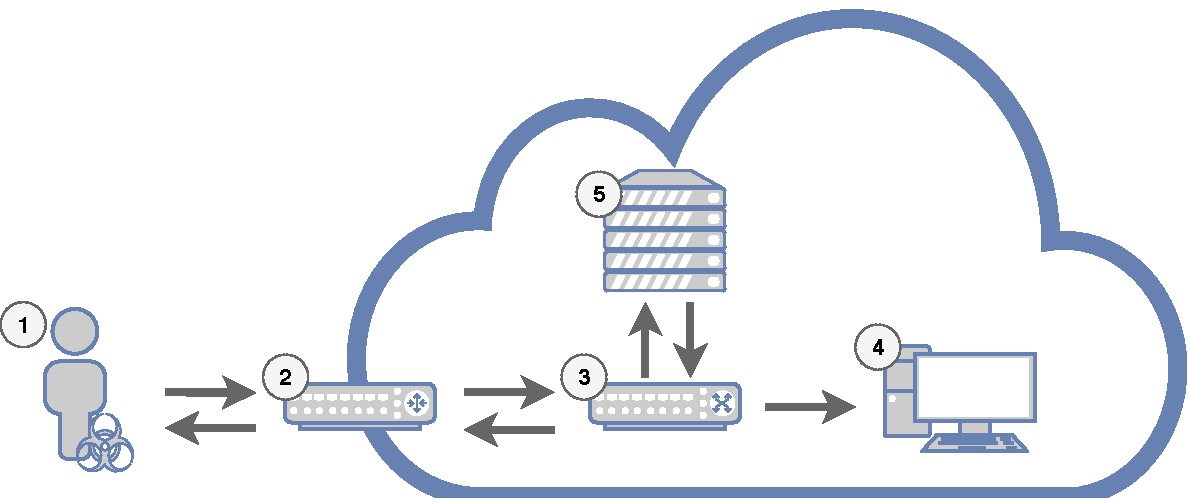
\includegraphics[width=\textwidth]{./images/test-setup.pdf}
\caption{Schematic overview test setup}
\end{figure}\label{fig:test-setup}

For this research, we choose 13 attack vectors retrieved from DDoSDB to test against our setup. Each vector has a pcap file which contains only the data belonging to this vector extracted from a real attack. From this, DDoSDB generated a JSON file which describes the main characteristics of that vector. Each vector has been assigned a four-digit identifier to which we refer to in the remainder of this paper. A brief summary of each attack vector based on the received JSON file can be found in Table \ref{tab:json-summarry}.  


\begin{table}[H]
\centering
\begin{tabular}{l | l | l | l | l | l}
ID & Type & \# src IPs & \# src ports & \# dst ports & special  \\ \hline \hline
e0b2 & ICMP & 83 & 0 & 0 & icmp\_type = 5 \\ \hline
0292 & TCP & 6 & 1 & 1 & tcp\_flags = ··········S· \\ \hline
dd26 & Chargen & 439 & 1 & 5 &  \\ \hline
e6ee & DNS & 25027 & 1 & 60219 & dns\_query = hoffmeister.be \\ \hline
54a7 & ICMP & 270 & 2821 & 1 & icmp\_type = 11 \\ \hline
8219 & UDP & 12 & 1 & 96 &  \\ \hline
39b6 & TCP & 66610 & 41757 & 1 & tcp\_flags = ············ \\ \hline
13c4 & UDP & 12 & 1 & 83 &  \\ \hline
c606 & TCP & 13452 & 12110 & 1 & tcp\_flags = ····CE····S· \\ \hline
7bf0 & NTP & 1288 & 1 & 11 &  \\ \hline
151e & ICMP & 244 & 12 & 1 & icmp\_type = 3 \\ \hline
9d61 & ICMP & 6245 & 0 & 0 & icmp\_type = 3 \\ \hline
072a & DNS & 30551 & 1 & 62591 & dns\_query = diasp.org
\end{tabular}
\caption{\label{tab:json-summarry}Attack charasterics}
\end{table}

A python script has been created that generates the signatures for the Bro SIDS. This script receives as input a JSON file received from DDoSDB and converts it to a valid Bro signature rule. Each attack vector has its own generated signature rule. For each vector the signature is generated on the Bro machine and is measured how long generation takes. The results of this can be found in Figure \ref{fig:generation-times}.

To measure the response time of the Bro SIDS against an ongoing DDoS attack, first, the maximum bandwidth of the target and Bro machines are determined. This is done using iperf3\footnote{\url{https://iperf.fr/}}. The attacker runs the script: \emph{iperf3 -s} and the other machine runs \emph{iperf3 -c [attacker\_ip] -R}. This way the server sends the data to the connecting machine. Second, the attacker will rewrite the destination IP and MAC-address of the supplied pcap using tcprewrite\footnote{\url{http://tcpreplay.synfin.net/}}. The command used is \emph{tcprewrite --dstipmap=0.0.0.0/0:[target\_ip]/32 --enet-dmac=[target\_mac] --infile=[supplied\_pcap] --outfile=attack.pcap}. Third, Bro is started in bare mode with the written Bro script described in Listing \ref{lst:bro-script}. This way only the needed files are loaded. The command used to start Bro is: \emph{sudo bro -b -i [network\_device] [path\_script]}. Fourth, the attack against the target machine is launched using tcpreplay. The command used to launch the attack is: \emph{sudo tcpreplay -i [network\_device] --mbps=[speed\_limit] attack.pcap}. Fifth and lastly, when a signature match is received, the Bro machine will send a message to the attacker. The times it took of each attack between launching it and receiving the message are displayed in Figure \ref{fig:attack-response-times}.



\section{Evaluation and Discussion}\label{subsec:evaluation-discussion}
In this section, we evaluate and discuss our findings we found by executing the methodology described in Section \ref{subsec:methodology}. We start by discussing the hardware used for the test setup and elaborate on each of the measured data.

In our first attempt at gathering results we used as the attacker a laptop with Intel i7-4700MQ @ 2.4 GHz with 8 GB of RAM running Ubuntu 18.04 LTS, as router the D-Link DIR-605L, as switch the tp-link TL-SG105E, as target machine a Raspberry Pi 2 and as Bro machine a Raspberry Pi 3 Model B. From iperf, we measured a maximum bandwidth of 90 Mbps. When replaying an attack vector at this rate, the Pi could not cope with it. We then decided to turn down the replay speed and concluded that even at a speed of 1 Mbps the Pi could not handle every attack. Therefore we concluded that a Pi, even for a signature set consisting of one signature, is not suitable to run the Bro SIDS.  

We then switched to using the attacking laptop as Bro machine and as attacker a different laptop. We again used iperf3 to measure the bandwidth that could be accomplished. This measured 90 Mbps.  

Several measurements were done during the experiment. Every measurement is executed 10 times. The first measurement performed is the time required to generate the Bro rules from the supplied JSON signatures. The results are shown in Figure \ref{fig:generation-times}. This figure shows the time it took in seconds to generate the signature on the Bro machine for each attack vector. As can be observed, the vectors e6ee, 072a and 39b6 took considerable more time than the other vectors. When combining this data with Table \ref{tab:attack-overview} we can conclude that the generation time grows with the number of entries.

\pgfplotstableset{
    create on use/mean/.style={create col/mean},
    create on use/stddev/.style={create col/standard deviation},
    create on use/stderror/.style={create col/standard error}
}

\begin{figure}[H]
\centering
\begin{tikzpicture}
  \begin{axis}[xticklabel style={rotate=90}, symbolic x coords={7bf0, 8219, c606, e6ee, 072a, e0b2, 9d61, 54a7, 151e, 0292, 39b6, 13c4, dd26, 7bf0, 8219, c606, e6ee, 072a, e0b2, 9d61, 54a7, 151e, 0292, 39b6, 13c4},
xtick={7bf0, 8219, c606, e6ee, 072a, e0b2, 9d61, 54a7, 151e, 0292, 39b6, 13c4, dd26, 7bf0, 8219, c606, e6ee, 072a, e0b2, 9d61, 54a7, 151e, 0292, 39b6, 13c4}, xticklabel style={text height=2ex}, xlabel={Attack Identifier}, ylabel={Time in seconds}, title={Bro Rule Generation Times},title style={xshift=1.5em, yshift=-1.5ex}]
    \addplot+[only marks, 
            error bars/.cd,
        y dir=both,
        y explicit
    ]
    table[
            x=Sample,
            y=mean,
            y error=stderror
    ]
    {results/data-generation.txt};
  \end{axis}
\end{tikzpicture}
\caption{Bro Rule Generation Times}
\label{fig:generation-times}
\end{figure}

The second measurement performed is the time it takes to send a message from the Bro machine to the attacker. The time measurement includes setting up a TCP connection, sending a message and then closing the connection. The average of these measurements was 8.41E-5 seconds with a standard error of 1.29E-5 seconds. 

The third and final measurement performed is the time it took for the Bro machine to react to an incoming attack. The results of these measurements are shown in Figure \ref{fig:attack-response-times}. This measurement is executed in two variants. The first variant is shown in Figure \ref{fig:attack-response-times-single} and pictures the response times when every attack vector has its own signature loaded in the Bro machine. The second variant shown in Figure \ref{fig:attack-response-times-all} pictures the response times when all attack vector's signatures are loaded. 

In Figure \ref{fig:attack-response-times-single} we observe that one vector, 39b6, takes less time than the other vectors. It is, however, visible that this measurement has quite a large variance compared to the other ones and might be that the reason for its speed is due to irregularities in the test setup. Furthermore, vectors 8219 and 13c4 take significantly longer to detect than the other attack vectors. It is interesting to note that both attack vectors are UDP attacks. One would more likely expect that the DNS attack vector would take longer to detect due to the fact that regex matching needs to be done against a packet's payload. Furthermore, the DNS attack vector e6ee has also more source IPs and destination ports to match against than both the UDP attacks. 

In Figure \ref{fig:attack-response-times-all} we observe that Bro does not increase significantly for all attack vectors. For most of the vectors, the times roughly stay the same. Most interesting are the increases in 072a and e0b2. Especially the latter as it increased by more than 2.5 times the time it took with only a single signature. Our initial guess was that this might be due to the order in which the rules were listed in the signature file. The order in the file was e0b2, 0292, dd26, e6ee, 54a7, 8219, 39b6, 13c4, c606, 7bf0, 151e, 9d61, 072a. From this, we conclude that the order is not what causes the increase in response time.  

\begin{figure}[H]
\centering
\begin{subfigure}[b]{0.5\linewidth}
\centering
\begin{tikzpicture}[yscale=0.7, xscale=0.7]
  \begin{axis}[xticklabel style={rotate=90}, symbolic x coords={7bf0, 8219, c606, e6ee, 072a, e0b2, 9d61, 54a7, 151e, 0292, 39b6, 13c4, dd26, 7bf0, 8219, c606, e6ee, 072a, e0b2, 9d61, 54a7, 151e, 0292, 39b6, 13c4},
xtick={7bf0, 8219, c606, e6ee, 072a, e0b2, 9d61, 54a7, 151e, 0292, 39b6, 13c4, dd26, 7bf0, 8219, c606, e6ee, 072a, e0b2, 9d61, 54a7, 151e, 0292, 39b6, 13c4}, xticklabel style={text height=2ex}, xlabel={Attack Identifier}, ylabel={Time in seconds}, title={Response Times Single Signature},title style={xshift=1.5em, yshift=-1.5ex}]
    \addplot+[only marks, 
            error bars/.cd,
        y dir=both,
        y explicit
    ]
    table[
            x=Sample,
            y=mean,
            y error=stderror
    ]
    {results/data-attacker-single-sigs.txt};
  \end{axis}
\end{tikzpicture}
\caption{Single Signatures}\label{fig:attack-response-times-single}
\end{subfigure}%
\begin{subfigure}[b]{0.5\linewidth}
\centering
\begin{tikzpicture}[yscale=0.7, xscale=0.7]
  \begin{axis}[xticklabel style={rotate=90}, symbolic x coords={7bf0, 8219, c606, e6ee, 072a, e0b2, 9d61, 54a7, 151e, 0292, 39b6, 13c4, dd26, 7bf0, 8219, c606, e6ee, 072a, e0b2, 9d61, 54a7, 151e, 0292, 39b6, 13c4},
xtick={7bf0, 8219, c606, e6ee, 072a, e0b2, 9d61, 54a7, 151e, 0292, 39b6, 13c4, dd26, 7bf0, 8219, c606, e6ee, 072a, e0b2, 9d61, 54a7, 151e, 0292, 39b6, 13c4}, xticklabel style={text height=2ex}, xlabel={Attack Identifier}, ylabel={Time in seconds}, title={Response Times All Signature},title style={xshift=1.5em, yshift=-1.5ex}]
    \addplot+[only marks, 
            error bars/.cd,
        y dir=both,
        y explicit
    ]
    table[
            x=Sample,
            y=mean,
            y error=stderror
    ]
    {results/data-attacker-all-sigs.txt};
  \end{axis}
\end{tikzpicture}
\caption{All signatures}\label{fig:attack-response-times-all}
\end{subfigure}
\caption{Graphs Showing response times after attack is launched}
\label{fig:attack-response-times}
\end{figure}









